% $Header: /home/vedranm/bitbucket/beamer/solutions/generic-talks/generic-ornate-15min-45min.en.tex,v 90e850259b8b 2007/01/28 20:48:30 tantau $
\documentclass{beamer}

%\documentclass[handout]{beamer}
%\usepackage{pgfpages}
%\usepackage{handoutWithNotes}
%\pgfpagesuselayout{2 on 1 with notes}[a4paper,landscape,border shrink=5mm]
% This file is a solution template for:

% - Giving a talk on some subject.
% - The talk is between 15min and 45min long.
% - Style is ornate.



% Copyright 2004 by Till Tantau <tantau@users.sourceforge.net>.
%
% In principle, this file can be redistributed and/or modified under
% the terms of the GNU Public License, version 2.
%
% However, this file is supposed to be a template to be modified
% for your own needs. For this reason, if you use this file as a
% template and not specifically distribute it as part of a another
% package/program, I grant the extra permission to freely copy and
% modify this file as you see fit and even to delete this copyright
% notice. 


\mode<presentation>
{
  \usetheme{Warsaw}
  % or ...

  \setbeamercovered{transparent}
  % or whatever (possibly just delete it)
}

\setbeamertemplate{navigation symbols}{} 

\usepackage[english]{babel}
% or whatever

\usepackage[latin1]{inputenc}
% or whatever

\usepackage{times}
\usepackage[T1]{fontenc}
% Or whatever. Note that the encoding and the font should match. If T1
% does not look nice, try deleting the line with the fontenc.


\title[Introduction to Python] % (optional, use only with long paper titles)
{Lecture 2}

\subtitle
{Introduction to Python} % (optional)

\author[Ying-Jer Kao] % (optional, use only with lots of authors)
{Ying-Jer Kao}
% - Use the \inst{?} command only if the authors have different
%   affiliation.

\institute[National Taiwan University] % (optional, but mostly needed)
{
  Department of Physics\\
 National Taiwan University
  }
% - Use the \inst command only if there are several affiliations.
% - Keep it simple, no one is interested in your street address.

\date[Numerical Analysis and Programming] % (optional)
{March 3, 2011}

\subject{Talks}
% This is only inserted into the PDF information catalog. Can be left
% out. 



% If you have a file called "university-logo-filename.xxx", where xxx
% is a graphic format that can be processed by latex or pdflatex,
% resp., then you can add a logo as follows:

% \pgfdeclareimage[height=0.5cm]{university-logo}{university-logo-filename}
% \logo{\pgfuseimage{university-logo}}



% Delete this, if you do not want the table of contents to pop up at
% the beginning of each subsection:
%\AtBeginSubsection[]
%{
%  \begin{frame}<beamer>{Outline}
%    \tableofcontents[currentsection,currentsubsection]
%  \end{frame}
%}


% If you wish to uncover everything in a step-wise fashion, uncomment
% the following command: 

%\beamerdefaultoverlayspecification{<+->}


\begin{document}

\begin{frame}
  \titlepage
\end{frame}

\begin{frame}{Outline}
  \tableofcontents
  % You might wish to add the option [pausesections]
\end{frame}


% Since this a solution template for a generic talk, very little can
% be said about how it should be structured. However, the talk length
% of between 15min and 45min and the theme suggest that you stick to
% the following rules:  

% - Exactly two or three sections (other than the summary).
% - At *most* three subsections per section.
% - Talk about 30s to 2min per frame. So there should be between about
%   15 and 30 frames, all told.

\section{Introduction}
\subsection[Goals of the course]{Goals of the course}

\begin{frame}{Goals of the course}{}
  % - A title should summarize the slide in an understandable fashion
  %   for anyone how does not follow everything on the slide itself.

  \begin{itemize}[<+->]
  \item
   \alert{ Problem solving skills}: the ability to formulate
problems, think creatively about solutions, and express a solution clearly
and accurately. 
      \item \alert{Learning  to program}:  an 
excellent opportunity to practice problem-solving skills.
\item \alert{Solving realistic physical problems}: make things interesting!!
\item We will use Python as our platform to achieve these goals. 
  \end{itemize}
\end{frame}

\subsection[What is Python?]{What is Python?}
\begin{frame}{What is Python?}
Python is an elegant and robust programming language that co	 flexibility of traditional compiled languages with the ease-of-use of simpler scripting and interpreted languages.
\begin{columns}
\column[t]{5.5cm}
\begin{itemize}
\item High-level 
\item Interpreted 
\item Scalable 
\item Extensible 
\item Portable 
\end{itemize}
\column[t]{5.5cm}
\begin{itemize}
\item Easy to learn, read and maintain 
\item Robust
\item Object Oriented 
\item Versatile
\end{itemize}
\end{columns}
\end{frame}

\begin{frame}{Why Python?}
\begin{itemize} 
\item Free \& open source
\item Available on a wide variety of platforms 
\item Better support for arrays with more than 2 dimensions 
\item Better support for wrapping FORTRAN 77/90/95 \& C/C++ code
\item Better memory management 
\item Much wider library support for non-numerical work 
\item More options for a full featured GUI
\item Easier to create stand-alone applications on any platform
\item Truly Object Oriented
\end{itemize}
\end{frame}

\begin{frame}{Why Python?}
\begin{itemize} [<+->]
\item It's easy to learn
\item Structure and syntax are pretty intuitive and easy to grasp
\item Excellent first programming language
\item Scientific Libraries 
\begin{itemize} 
\item \alert{numpy}: Linear algebra
\item \alert{scipy}: Optimization, ODEs, Fourier, etc.
\item \alert{matplotlib}: 2D Plotting
\end{itemize}
\end{itemize}
\end{frame}
\begin{frame}{The Python Programming Language}{}
\begin{itemize}
 \item Python is an example of a {\bf high-level language}.
 \item   Some other high-level languages: C, C++, Perl, and Java.
\end{itemize}
\begin{block}
%\begin{itemize} 
{Traditional languages (C++, Java)} 
Evolved for large-scale
programming 
\begin{itemize}
\item Emphasis on \alert{structure and discipline} 
\item Simple problems $\ne$ simple programs
\end{itemize}

\end{block}
\begin{block}{Scripting languages (Perl, Python)}
 Designed for
simplicity and flexibility
\begin{itemize}
\item Simple problems = simple, elegant solutions 
\item More amenable to \alert{experimentation and incremental development}
\end{itemize}
\end{block}
\end{frame}


\begin{frame}[fragile]
\frametitle{Hello World ! (C++)}
  % - A title should summarize the slide in an understandable fashion
  %   for anyone how does not follow everything on the slide itself.
\begin{verbatim}
#include <iostream>
using namespace std;
int main()
{
  cout << "Hello, World!" << endl;  
}
\end{verbatim}  
\end{frame}

\begin{frame}[fragile]
\frametitle{ Hello World ! (Python) }
In IDLE,
\begin{verbatim}
>>> print "Hello World!"
\end{verbatim}
\vspace*{0.1in}
or as a file, 
\begin{verbatim}
#!/usr/bin/python
print "Hello World!"
\end{verbatim}
\begin{itemize}
\item Some people judge the quality of a programming language by the simplicity of the ``Hello, World!'' program. 
\item By this standard, Python does about as well as possible.
\end{itemize}
\end{frame}
\begin{frame}{Interpreter and Compiler}
Two kinds of programs process high-level languages into low-level languages: \alert{interpreters and compilers}.
\begin{itemize}[<+->]
\item An interpreter reads a high-level program and executes it.
\item It processes the program a little at a time, alternately reading lines and performing computations.
\end{itemize}
\vspace*{0.2in}
\centerline{\includegraphics[height=0.77in]{thinkpython/figs/interpret.eps}}
\end{frame}

\begin{frame}{Interpreter and Compiler}
\begin{itemize}[<+->]
\item A compiler reads the program and translates it completely before the program starts running. 
\item The high-level program is called the \alert{source code}.
\item The translated program is called the \alert{object code} or the \alert{executable}. 
\item Once a program is compiled, you can execute it repeatedly without further translation.
\end{itemize}
\vspace*{0.2in}
\centerline{\includegraphics[height=0.77in]{thinkpython/figs/compile.eps}}

\end{frame}

\begin{frame}
Python is considered an \alert{interpreted language} because Python programs
are executed by an interpreter.
\begin{itemize}
\item Rapid turnaround: no intermediate compile and link steps as in C or C++
\item Hybrid Python programs are compiled automatically to an intermediate form called \alert{bytecode}, which the interpreter then reads
\item This gives Python the development speed of an interpreter without the performance loss inherent in purely interpreted languages
\end{itemize}
\end{frame}

\begin{frame}{Running Programms in Python}

To run a Python program, one can
\begin{itemize}
\item Start interpreter from command line 
\begin{itemize}
\item Type program statements
\item Import script file
\end{itemize}
\item Start interpreter with file as command line arg 
\item Configure filetype to launch interpreter on file
\item Unix/Linux "\#!" trick 
\item \alert{Directly from IDE (IDLE)}
\end{itemize}
\end{frame}
\section{Programming}
\subsection{Program}
\begin{frame}{What is a Program?}
A {\bf program} is a sequence of instructions that specifies how to
perform a computation
\begin{itemize}[<+->]
\item Mathematical computation
\begin{itemize}
\item solving a system of equations
\item finding the
roots of a polynomial
\end{itemize}
\item Symbolic computation
\begin{itemize}
\item searching and replacing text in a document
\item compiling a program
\end{itemize}
\end{itemize}
\end{frame}
\begin{frame}{Structure of a Program}
\begin{itemize}
\item \textbf{input}: Get data from the keyboard, a file, or some
other device.
\item \textbf{output}: Display data on the screen or send data to a
file or other device.
\item \textbf{math}: Perform basic mathematical operations like addition and
multiplication.
\item \textbf{conditional execution}: Check for certain conditions and
execute the appropriate sequence of statements.
\item \textbf{repetition}: Perform some action repeatedly, usually with
some variation.
\end{itemize}
\end{frame}

\begin{frame}{Bugs and Debugging}

\begin{block}{Programming}
\begin{itemize}
\item Programming is \alert{error-prone}.
\item Programming errors are called \alert{bugs}. 
\item The process of tracking them down is called \alert{debugging}.
\end{itemize}
\end{block}
\begin{block}{Types of Errors}
\begin{itemize}
\item Syntax errors
\item Runtime errors
\item Semantic errors
\end{itemize}
\end{block}
\end{frame}
\begin{frame}{Bug}
\centerline{\includegraphics[height=3.5in]{bug.jpg}}
\end{frame}
\subsection{Syntax errors}
\begin{frame}{Syntax Errors}
\textbf{Syntax}--
\begin{itemize}
\item The structure of a program and the rules about that structure.
\item What statements are legal?
\end{itemize}
\begin{block}{Example: parenthses}
\begin{itemize}
\item \texttt{(1+2)} is legal.
\item \texttt{8)} is a \alert{syntax error}.
\end{itemize}
\end{block}
\end{frame}

\begin{frame}[fragile]
\frametitle{Syntax Errors}
If there is a \alert{single syntax error} anywhere in your program, Python will display an error message and quit.
\begin{block}{hello\_syntax\_error.py}
\begin{verbatim}
print 'Hello, Physics!
\end{verbatim}
\end{block}\pause
\begin{block}{}
\begin{verbatim}
$python hello_syntax_error.py 
  File "hello_syntax_error.py", line 3
    print 'Hello, Physics!
                         ^
SyntaxError: EOL while scanning string literal
\end{verbatim}
\end{block}
\end{frame}
%
%Python can only execute a program if the syntax is
%correct; otherwise, the interpreter displays an error message.
%{\bf Syntax} refers to the structure of a program and the rules about
%that structure. \index{syntax} 
%For example, parentheses have to come in matching pairs, so
%{\tt (1 + 2)} is legal, but {\tt 8)} is a {\bf syntax error}.
%
%
%
%In English readers can tolerate most syntax errors, which is why we
%can read the poetry of e. e. cummings without spewing error messages.
%Python is not so forgiving.  If there is a single syntax error
%anywhere in your program, Python will display an error message and quit,
%and you will not be able to run your program. During the first few
%weeks of your programming career, you will probably spend a lot of
%time tracking down syntax errors.  As you gain experience, you will
%make fewer errors and find them faster.
%
\subsection{Runtime errors}
\begin{frame}[fragile]
\frametitle{Runtime Errors}
\begin{itemize}
\item Runtime errors do not appear until after the program has started running.
\item Also called \alert{exceptions}. Exceptions can be handled in Python programs.
\item Exceptions not handled by the program will result in error messages.
\end{itemize}
\begin{block}{Examples}
\begin{semiverbatim}
>>> 10 * (1/0)\pause
Traceback (most recent call last):
  File "<stdin>", line 1, in ?
ZeroDivisionError: integer division or modulo 
by zero
\end{semiverbatim}
\end{block}
\end{frame}


%These errors are also called {\bf exceptions} because they usually
%indicate that something exceptional (and bad) has happened.
%
%Runtime errors are rare in the simple programs you will see in the
%first few chapters, so it might be a while before you encounter one.
%
%\end{frame}
%
\subsection{Semantic errors}
\begin{frame}{Semantic Errors}
\begin{itemize}[<+->]
\item  The program  will \alert{run successfully} without generating any error messages, but it \alert{will
not} do the right thing. 
\item It does something else.
\item It does \alert{exactly} what you told it to do. 
\item The program you wrote does not corresponding to the program you \alert{wanted to write}.
\item \alert{Most difficult} to debug.
\item Developing \alert{good programming style} will help reduce the occurrence of semantic errors.
\end{itemize}
\end{frame}

\section{Variables, Expressions and Statements}
\subsection{Values and Types}

\begin{frame}[fragile]
\frametitle{Values and Types}
A \alert{value} is one of the basic things a program works with, like a \alert{number} or \alert{letter}.  
\begin{block}{Examples}
\begin{itemize}
\item \texttt{1}, \texttt{2}
\item \verb"'Hello, World!'"
\end{itemize}
\end{block}
They belong to different \alert{types}
\begin{itemize}
\item \texttt{ 2} is an \alert{integer}, 
\item \verb"'Hello, World!'" is a \alert{ string}.
\end{itemize}
\end{frame}
\begin{frame}[fragile]
\frametitle{Finding Out the Type}
If you are not sure what type a value has, the interpreter can tell you.
\begin{verbatim}
>>> type('Hello, World!')
<type 'str'>
>>> type(17)
<type 'int'>
>>> type(3.2)
<type 'float'>
\end{verbatim}
\end{frame}
\begin{frame}[fragile]
\frametitle{Types}
Built-in types in Python
\begin{block}{Numbers}
\begin{itemize} 
\item  Integer: \verb"1234"
\item Long Integer: \verb"123151242345234523452345L"
\item Float:  \verb"3.1415"
\item Complex: \verb"3+4j"
\end{itemize}
\end{block}
\begin{block}{Strings}
\verb!'spam', "python"!
\end{block}
\end{frame}
\begin{frame}[fragile]
\frametitle{Types}
\begin{block}{Lists}
\verb![1, [2, 'three'], 4]!
\end{block}
\begin{block}{Tuples}
\verb!(1, 'spam', 4, 'U')!
\end{block}
\begin{block}{Dictionaries}
\verb!{'food' : 'spam', 'taste' : 'yum'}!
\end{block}
\begin{block}{Sets}
\verb!{'a','b','c'}!
\end{block}
\end{frame}
\subsection{Variables}
\begin{frame}[fragile]
\frametitle{Variables}
\begin{itemize}
\item \textbf{Variable}:  a name that refers to a value.
\item \textbf{Assignment Statement}: creates new variables and gives
them values
\end{itemize}
{\tiny
\begin{verbatim}
>>> message = 'And now for something completely different'
>>> n = 17
>>> pi = 3.1415926535897931
\end{verbatim}}

\vspace*{0.1in}
A common way to represent variables  is to write the name with
an arrow pointing to the variable's value.
\vspace*{0.15in}
\centerline{\includegraphics{thinkpython/figs/state2.eps}}
\end{frame}
\begin{frame}[fragile]
\frametitle{Using Variables}
\begin{verbatim}
>>> print n
17
>>> print pi
3.14159265359
>>> x=pi
>>> print x
3.14159265359
\end{verbatim}
\end{frame}
\begin{frame}[fragile]
\frametitle{Types of Variables}
\begin{verbatim}
>>> type(message)
<type 'str'>
>>> type(n)
<type 'int'>
>>> type(pi)
<type 'float'>
\end{verbatim}
\end{frame}
%
%
\begin{frame}[fragile]
\frametitle{Dynamic Typing}
\begin{itemize}
\item Type of a variable is associated to the \alert{value}
\begin{verbatim}
>>> x =3
>>> type(x)
<type 'int'>
>>> x='3'
<type 'str'>
\end{verbatim}
\item  \alert{Do not} change the type of a variable.
\end{itemize}
\end{frame}
%
\begin{frame}[fragile]
\frametitle{Variable Names and Keywords}
\begin{itemize}[<+->]
\item Choose meaning names of variables indicating what the variable is used for.
\item Variable names can be arbitrarily long.
\item Can be with both letters and numbers, but have to start with a letter.
\item It is a good idea to begin variable names with a  \alert{lowercase letter}.
\item The underscore character (\verb"_") can appear in a name. For example, 
\verb"my_name" or \verb"airspeed_of_unladen_swallow".
\end{itemize}
\end{frame}

\begin{frame}[fragile]\frametitle{Illegal Names}
If you give a variable an illegal name, you get a syntax error:
\begin{block}{}
\begin{verbatim}
>>> 76trombones = 'big parade'
SyntaxError: invalid syntax
>>> more@ = 1000000
SyntaxError: invalid syntax
>>> class = 'Advanced Theoretical Zymurgy'
SyntaxError: invalid syntax
\end{verbatim}
\end{block}
\end{frame}
%
\begin{frame}[fragile]
\frametitle{Keywords}
\begin{itemize}
\item
Python has 31 keywords
\begin{block}{Keywords}
\begin{verbatim}
and       del       from      not       while    
as        elif      global    or        with     
assert    else      if        pass      yield    
break     except    import    print              
class     exec      in        raise              
continue  finally   is        return             
def       for       lambda    try
\end{verbatim}
\end{block}
\item
The
interpreter uses keywords to recognize the structure of the program,
and they cannot be used as variable names.
\end{itemize}
\end{frame}
\subsection{Statements}
\begin{frame}[fragile]\frametitle{Statements}
A statement is a unit of code that the Python interpreter can
execute.  
\begin{block}{}
\begin{verbatim}
print 1 #print an integer value
x = 2   #assign value 2 to x
print x #print the value of x
\end{verbatim}
\end{block}
\begin{block}{Output}
\begin{verbatim}
1
2
\end{verbatim}
\end{block}
\end{frame}
\subsection{Operators and operands}
\begin{frame}[fragile]
\frametitle{Operators and Operands}
\begin{itemize}
\item \textbf{Operators}: special symbols that represent computations like
addition and multiplication.  
\item \textbf{Operands} : the values the operator is applied to
\end{itemize}
\begin{block}{Operators}
\begin{itemize} 
\item \texttt{+}: addition
\item \texttt{-}: subtraction
\item  \texttt{*}: multiplication
\item \texttt{/}: division
\item \texttt{**}: exponentiation
\end{itemize}
\end{block}
\end{frame}
\begin{frame}[fragile]
\frametitle{Expression}

\textbf{Expression}: combination of values, variables, and operators.
\begin{block}{Examples}
\begin{verbatim}
17
x
x + 17
\end{verbatim}
\end{block}
\begin{block}{Interactive Mode/Script}
\begin{verbatim}
>>> 1+1
2
\end{verbatim}
\end{block}
\end{frame}
\begin{frame}[fragile]
\frametitle{Arithmetic Operations}
\begin{itemize}
\item Unary Arithmetic Operations
\begin{center}
\begin{verbatim}
expr ::= op A
\end{verbatim}
\end{center}
\begin{block}{Operators}
\begin{itemize}
\item \texttt{-},  \texttt{+} 
\end{itemize}
\end{block}
\item Binary Arithmetic Operations
\begin{center}
\begin{verbatim}
expr ::= A op B
\end{verbatim}
\end{center}
\begin{block}{Operators}
%\begin{columns}
%\column[t]{4.5cm}
\begin{itemize}
\item \texttt{+, -}
\item \texttt{*, /, //, \%} 
\item \texttt{**} 
\end{itemize}
%\column[t]{4.5cm}
%\begin{itemize}
%\item \texttt{<, >, <=, >=}
%\item \texttt{==, !=}
%\end{itemize}
%\end{columns}
\end{block}
\end{itemize}
\end{frame}
\begin{frame}[fragile]
\frametitle{Digression: Division, Modulo }

\begin{block}{}
\begin{itemize}
\item \texttt{/}: division
\begin{verbatim}
>>> 5 / 2 = 2 (Python 2.x)
>>> 5 / 2 = 2.5  (Python 3.x)
\end{verbatim}
\item For Python 2.x, dividing two integers or longs uses integer division, also known as \alert{floor division}, and \alert{true division} for all other types. For Python 3.x, \texttt{/} does \alert{true division} for all types.
\end{itemize}
\end{block}
\begin{block}{\texttt{//}: floor division}
\begin{itemize}
\item Applying the floor function after division.
\begin{verbatim}
>>> 5 // 2 = 2
>>> 5.0 // 2 = 2.0
\end{verbatim} 
\end{itemize}
\end{block}
\end{frame}
\begin{frame}[fragile]
\frametitle{Digression: Division, Modulo }

\begin{block}{ \texttt{\%}: modulo}
\begin{itemize}
\item Gives the remainder of a division. 
\begin{verbatim}
>>> 5 % 2 = 1
>>> 5.0 % 2 = 1.0
\end{verbatim}
\item Integer division and modulo operators are connected by $x== ( x / y )*y+x \% y$
\item Built-in function \texttt{divmod(x,y)}: gives \texttt{ (x/y, x\%y)} 
\end{itemize}
\end{block}
Things get tricky when the divisor is negative. (Lab)
\end{frame}


\begin{frame}[fragile]
\frametitle{Operator  Precedence}
How does Python evaluate \verb! A * B + C * D =!?

\begin{itemize}
\item Mixed operators are evaluated following operator precedence.
\item \alert{ PEMDAS} rules: \textit{Parentheses, Exponentiation, Multiplication, Division, Addition, Subtraction} 
%\begin{block}{Operator Precedence of }
%\begin{itemize}
%\item \texttt{()}
%\item \texttt{**}
%\item \texttt{*},\texttt{/}
%\item \texttt{+},\texttt{-}
%\end{itemize}
%\end{block}
\item  Operators with the same precedence are evaluated from \alert{left to 
right}. 
\item When in doubt, use parentheses ().
\end{itemize}
\end{frame}
\begin{frame}[fragile]
\frametitle{Operator  Precedence}
\centerline{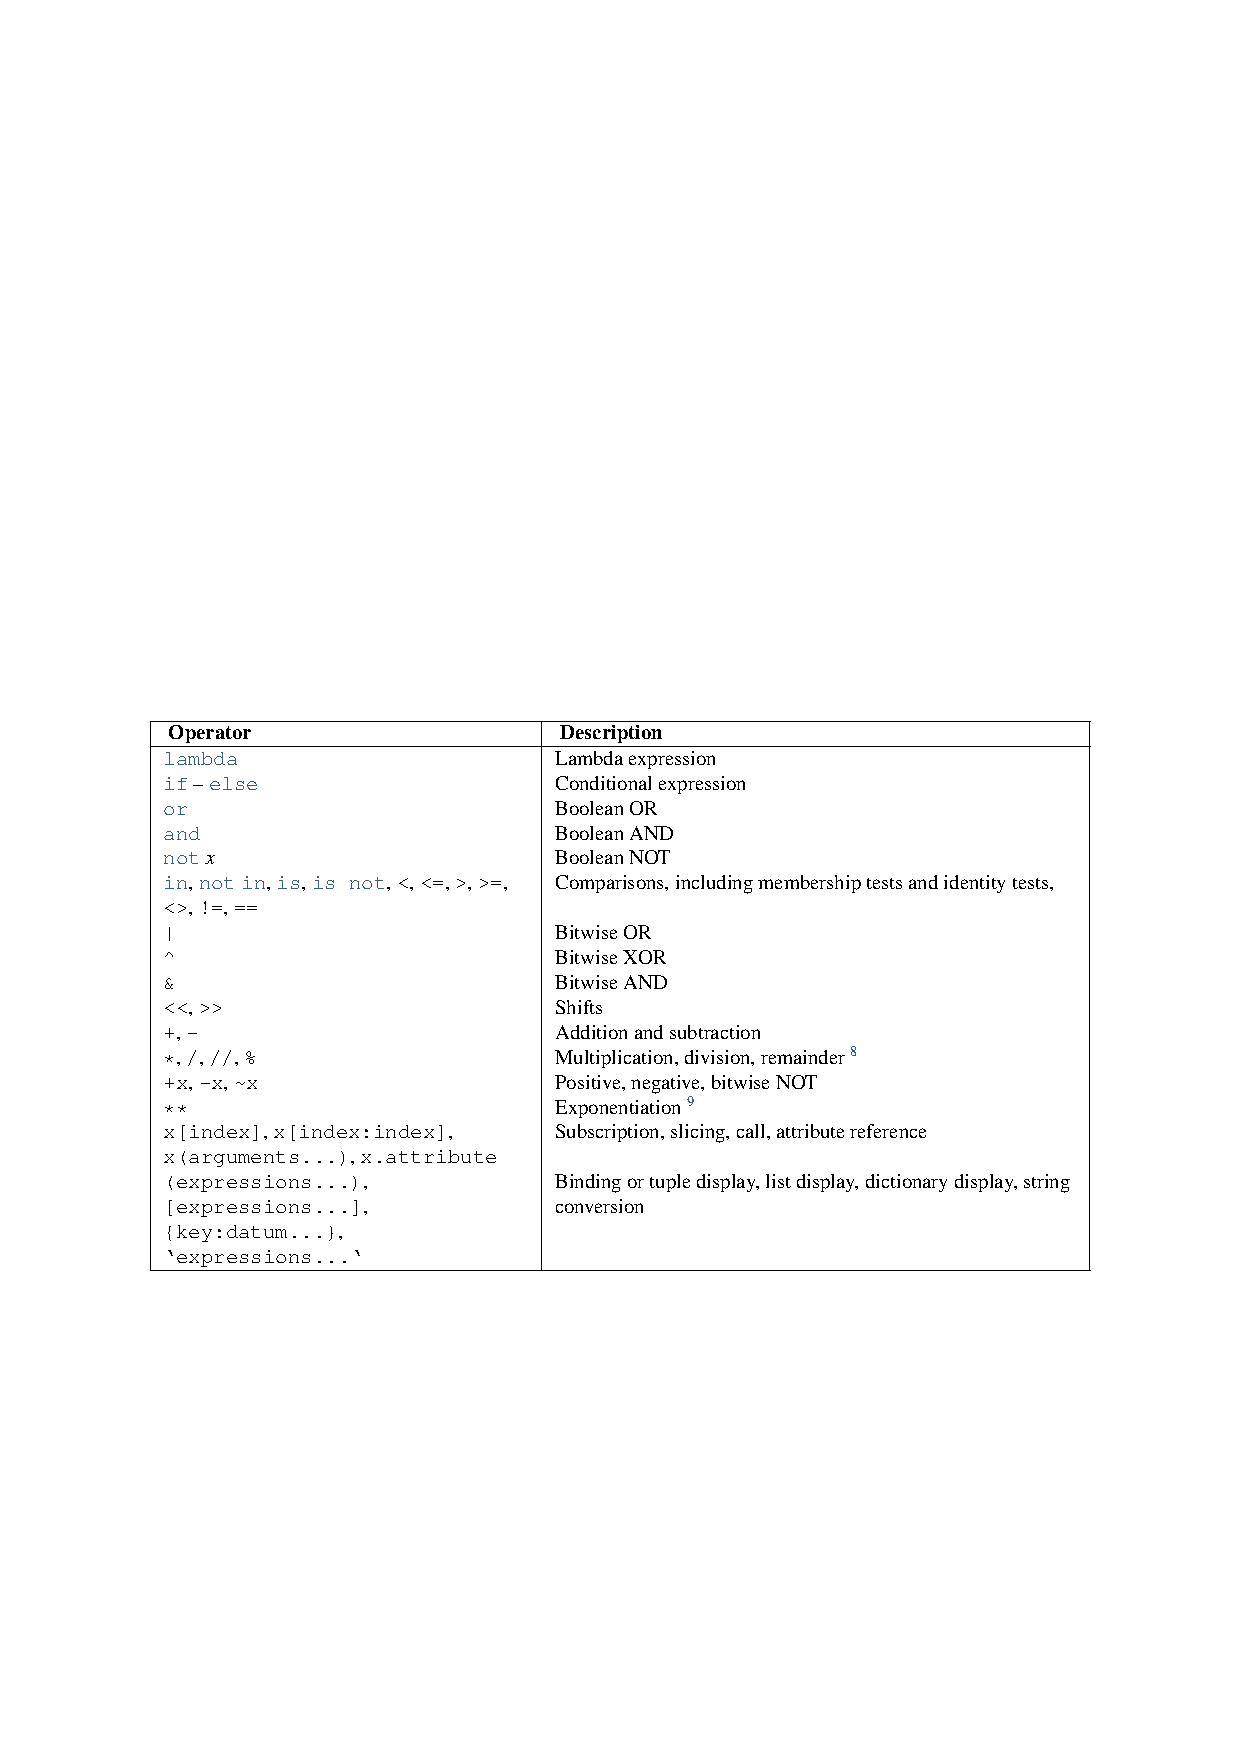
\includegraphics[width=\textwidth]{operator_precedence}}
\end{frame}

\begin{frame}[fragile]

\frametitle{String operations}
\begin{itemize}
\item Illegal statements:
\begin{verbatim}
'2'-'1'  'eggs'/'easy' 'third'*'a charm'
\end{verbatim}

\item \texttt{+}:  \alert{concatenation}\\
 Joining the strings by
linking them end-to-end
%\begin{block}{example}
%\begin{columns}
%\column[t]{4cm}
%Code:
%\begin{verbatim}
%first = 'throat'
%second = 'warbler'
%print first + second
%\end{verbatim}
%\column[t]{4cm}
%Output: \texttt{throatwarbler}
%\end{columns}
%\end{block}
\item \texttt{*}:  \alert{repetition}\\
 If one of the operands is a \alert{string}, the other has to be an \alert{integer}.
\end{itemize}
\end{frame}
\begin{frame}[fragile]
\frametitle{Comments}
\begin{itemize}
\item As programs get bigger and more complicated, they get more \alert{difficult
to read}.  
\item It is a good practice to add \alert{comments} to explain
in human language what the program is doing.  
\item In Python, they start with the \verb"#" symbol.
\end{itemize}
\end{frame}
\begin{frame}[fragile]
\frametitle{Comments}
\begin{itemize}
\item Comments can appear on a line.
\begin{block}{}
\tiny
\begin{verbatim}
# compute the percentage of the hour that has elapsed
percentage = (minute * 100) / 60
\end{verbatim}
\end{block}

\item They can also appear at the end of a line
\begin{block}{}
\tiny
\begin{verbatim}
percentage = (minute * 100) / 60     # percentage of an hour
\end{verbatim}
\end{block}
\item Everything from the \texttt{\#} to the end of the line is \alert{ignored}.
\end{itemize}
\end{frame}


\begin{frame}[fragile]
\frametitle{Comments}
\begin{itemize}
\item Comments are most useful when they document \alert{non-obvious} features of
the code. 
\item It is much more useful to explain \alert{why} as supposed to \alert{what}.

\begin{block}{Useless comment}
\small
\begin{verbatim}
v = 5     # assign 5 to v
\end{verbatim}
\end{block}
%
%This comment contains useful information that is not in the code:
\pause
\begin{block}{Useful information not in the code}
\small
\begin{verbatim}
v = 5     # velocity in meters/second. 
\end{verbatim}
\end{block}
\item Some argue \alert{half} of your code should be comments.
\end{itemize}
\end{frame}
%
%
%The third type of error is the {\bf semantic error}.  If there is a
%semantic error in your program, it will run successfully in the sense
%that the computer will not generate any error messages, but it will
%not do the right thing.  It will do something else.  Specifically, it
%will do what you told it to do.
%
%The problem is that the program you wrote is not the program you
%wanted to write.  The meaning of the program (its semantics) is wrong.
%Identifying semantic errors can be tricky because it requires you to work
%backward by looking at the output of the program and trying to figure
%out what it is doing.

%\begin{frame}{Make Titles Informative.}
%
%  You can create overlays\dots
%  \begin{itemize}
%  \item using the \texttt{pause} command:
%    \begin{itemize}
%    \item
%      First item.
%      \pause
%    \item    
%      Second item.
%    \end{itemize}
%  \item
%    using overlay specifications:
%    \begin{itemize}
%    \item<3->
%      First item.
%    \item<4->
%      Second item.
%    \end{itemize}
%  \item
%    using the general \texttt{uncover} command:
%    \begin{itemize}
%      \uncover<5->{\item
%        First item.}
%      \uncover<6->{\item
%        Second item.}
%    \end{itemize}
%  \end{itemize}
%\end{frame}
%
%
%\subsection{Second Subsection}
%
%\begin{frame}{Make Titles Informative.}
%\end{frame}
%
%\begin{frame}{Make Titles Informative.}
%\end{frame}
%
%
%
%\section*{Summary}
%
%\begin{frame}{Summary}
%
%  % Keep the summary *very short*.
%  \begin{itemize}
%  \item
%    The \alert{first main message} of your talk in one or two lines.
%  \item
%    The \alert{second main message} of your talk in one or two lines.
%  \item
%    Perhaps a \alert{third message}, but not more than that.
%  \end{itemize}
%  
%  % The following outlook is optional.
%  \vskip0pt plus.5fill
%  \begin{itemize}
%  \item
%    Outlook
%    \begin{itemize}
%    \item
%      Something you haven't solved.
%    \item
%      Something else you haven't solved.
%    \end{itemize}
%  \end{itemize}
%\end{frame}


\end{document}


